\documentclass{article}

\usepackage[margin=1in]{geometry}
\usepackage{amsfonts}
\usepackage{amssymb}
\usepackage{mathtools}
\usepackage{graphicx}
\graphicspath{ {./} }
\linespread{2}

\begin{document}

\title{	CMSC 471 -- Project 3\\ 
	Image Classification}
\author{Jeremy Aguillon}

\maketitle

\newpage

\section{Pickling}

The given data set was very large and difficult to deal with all at once. Because of this, I decided to parse the data and perform the featurization on each image once. To do this, I loop through each of the given folders to featurize each of the images and gather the labels. It was impossible to tell whether or not this was working, simply by looking at the code and the output produced from the code. So as I was storing each of the featurized images, I created a subplot with matplotlib to print out an image to the screen with its label to prove that the correct label and images were being matched. After both the images and the labels are stored in two lists and I pickle the data as 1 2-element list containing both data lists. This provides much more generalizability, because my program can use any pickle file in this format without changing anything.

\section{Training the Model}

Once the data has been featurized and pickled, it is available via unpickling in any of my other programs. Following data parsing, the next step was to choose and train the model. I decided on scikit learn tools because their interface is very straightforward and fits the requirements of this project perfectly. I initially trained the data using 10 of each pictures and labels. I chose the model of Support Vector Machine, because it was the first one in the examples and one of the first ones we spoke about in class. However, when I began testing this it was not accurate at all and would consistently predict incorrectly. So, I began reading more advanced scikit learn examples and found that there was a built in method of separating your data into training and test data. So, instead of only importing 10 or 20 images each and testing on the rest, I imported all of the images and put them through the train\_test\_split() function provided by scikit learn and it produced data sets that I could easily plug in and use. After doing, this I still was not happy with how the model was performing I decided to switch to the K Nearest Neighbor model. The K Nearest Neighbor model was equally as intuitive as the Support Vector Machine, however it performed much better on my initial tests. 


\section{Testing the Accuracy}

I thought that the Support Vector Machine performed worse than the K Nearest Neighbor model, but I wanted to be sure. To do this, I created confusion matrices for both of them from the same data set. 

	\begin{figure}[!htb]
		\centering
		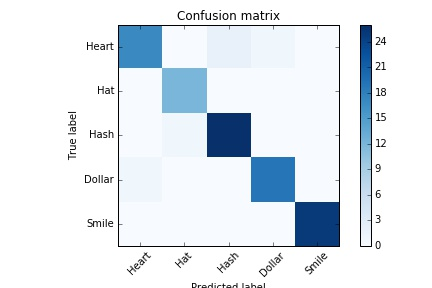
\includegraphics[scale=.5]{SVM_CM.jpg}
		\caption{A non-normalized confusion matrix for the Support Vector Machine model}
		\label{SVM_CM}
	\end{figure}	
	
	\begin{figure}[!htb]
		\centering
		\begin{tabular}{|l|c|c|c|c|c|} 
			\hline 
			& Heart & Hat & Hash & Dollar & Smile \\
			\hline
			Heart & 17 & 0 & 2 & 1 & 0 \\
			Hat & 0 & 12 & 0 & 0 & 0 \\
			Hash & 0 & 1 & 26 & 0 & 0 \\
			Dollar & 1 & 0 & 0 & 19 & 0 \\
			Smile & 0 & 0 & 0 & 0 & 25 \\
			\hline
		\end{tabular}
		\caption{Table showing statistics generated in the Support Vector Machine Confusion Matrix}
		\label{SVM_Data}
	\end{figure}
		
	Here are the results from the Support Vector Machine on the data set that was split by the scikit learn function shown in Figures \ref{SVM_CM} and \ref{SVM_Data}. As you can see, the model is quite accurate and has only had 4 incorrect guesses out of 103 images. However, I was determined to have a higher accuracy and switched models after this. 
	
	\newpage
	
	\begin{figure}[!htb]
		\centering
		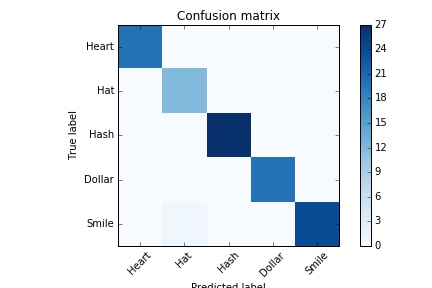
\includegraphics[scale=.5]{KNN_CM.jpg}
		\caption{A non-normalized confusion matrix for the K Nearest Neighbor model}
		\label{fig:KNN_CM}
	\end{figure}
	
	\begin{figure}[!htb]
		\centering
		\begin{tabular}{|l|c|c|c|c|c|} 
			\hline 
			& Heart & Hat & Hash & Dollar & Smile \\
			\hline
			Heart & 20 & 0 & 0 & 0 & 0 \\
			Hat & 0 & 12 & 0 & 0 & 0 \\
			Hash & 0 & 0 & 27 & 0 & 0 \\
			Dollar & 0 & 0 & 0 & 20 & 0 \\
			Smile & 0 & 1 & 0 & 0 & 24 \\
			\hline
		\end{tabular}
		\caption{Table showing statistics generated in the K Nearest Neighbor Confusion Matrix}
		\label{KNN_Data}
	\end{figure}
		
	As you can see in Figures \ref{fig:KNN_CM} and \ref{KNN_Data}, the K Nearest Neighbor model clearly outperforms the Support Vector Machine model. While it may seem going from 97\% accuracy to 99\% accuracy is small, I believe in this case it is quite significant because the classification level is almost perfect and works very well on all pictures it is given. 
	
\end{document}